\chapter{Applications linéaires et calcul matriciel}

\section{Applications linéaires entre $\R^n$ et $\R^p$}

\subsection{Définition, exemples}
Après avoir beaucoup travaillé dans $\R^n$ à résoudre des systèmes linéaires et à multiplier des matrices et des vecteurs, il est naturel de se poser des questions sur les fonctions entre $\R^n$ et $\R^p$, ainsi que leurs propriétés. Nous n'allons pas étudier toutes les applications $T: \R^n \to \R^p$ possibles: en algèbre linéaire, seule une classe de ces applications nous intéressera, les \textit{applications linéaires}. 

Avant de donner la définition, il faut remarquer que les autres types d'applications sont quand même intéressants à étudier, mais ils demandent des outils qui proviennent d'autres domaines des mathématiques.

Voici la classe d'applications étudiée par l'algèbre linéaire:
\begin{boxdef}[Application Linéaire]
Une application $T: \R^n \to \R^p$ est dite \textit{linéaire} si et seulement si:
\begin{itemize}
    \item $\forall x,y \in \R^n$, $T(x+y) = T(x) + T(y)$
    \item $\forall \lambda \in \R$, $\forall x \in \R^n$, $T(\lambda x) = \lambda T(x)$
\end{itemize}
\end{boxdef}
Concrètement, une application linéaire est une application qui préserve les opérations $+$ et $\cdot$: sommer deux vecteurs puis appliquer $T$ est équivalent à d'abord appliquer $T$ ensuite sommer ces deux vecteurs. Le même raisonnement s'applique pour la multiplication d'un vecteur par un scalaire.

Donnons des exemples pour voir ce qu'est (et ce que n'est pas) une application linéaire:

Soit $T: \R^3 \to \R^2$ définie par:
$$x = \begin{bmatrix}
x_1 \\ x_2 \\ x_3
\end{bmatrix} \mapsto T(x) = 
\begin{bmatrix}
x_1 + x_3 \\ x_2
\end{bmatrix}$$
C'est une application linéaire. Pour le voir, il faut vérifier les deux propriétés de la définition:
\begin{align*}
    \forall x,y \in \R^3, T(x+y) &=
    \begin{bmatrix}
    (x+y)_1 + (x+y)_3 \\ (x+y)_2
    \end{bmatrix} \\
    &= \begin{bmatrix}
    x_1 + y_1 + x_3 + y_3 \\ x_2 + y_2
    \end{bmatrix} \\
    &= \begin{bmatrix}
    x_1 + x_3 \\ x_2
    \end{bmatrix} + \begin{bmatrix}
    y_1 + y_3 \\ y_2
    \end{bmatrix} 
    = T(x) + T(y)
\end{align*}
Ensuite, on a $\forall \lambda \in \R$ et $\forall x \in \R^3$:
\begin{align*}
    T(\lambda x) &= 
    \begin{bmatrix}
    \lambda x_1 + \lambda x_3 \\ \lambda x_2
    \end{bmatrix} \\ 
    &= \lambda \begin{bmatrix}
    x_1 + x_3 \\ x_2
    \end{bmatrix}
    = \lambda T(x)
\end{align*}

Pour donner un autre exemple, l'application $T: \R^2 \to \R^2$ définie comme suit n'est pas linéaire:
$$x = \begin{bmatrix} x_1 \\ x_2 \end{bmatrix} \mapsto T(x) = \begin{bmatrix} x_1 x_2 \\ 4x_1 \end{bmatrix}$$
En effet, $\forall \lambda \in \R$,
$$T(\lambda x) = \begin{bmatrix} \lambda x_1 \cdot \lambda x_2 \\ 4\lambda x_1\end{bmatrix} = \lambda \begin{bmatrix} \lambda x_1 x_2 \\ 4x_1 \end{bmatrix} \neq \lambda \begin{bmatrix}  x_1 x_2 \\ 4x_1 \end{bmatrix} = \lambda T(x)$$
Nous pouvons vérifier de la même manière que la première propriété de la définition n'est pas satisfaite non plus.

\subsection{Cas particulier: les applications matricielles}
Nous avons défini le produit matrice-vecteur dans la partie \ref{definitionProduitMatVec}, et nous allons l'utiliser pour étudier les \textit{applications matricielles}, c'est-à-dire les applications de la forme
\begin{align*}
    T: \, &\R^n \to \R^p \\
    & x \mapsto Ax
\end{align*}
avec $A \in \R^{p \times n}$ une matrice. 

Nous énonçons ensuite un résultat  particulièrement intéressant:

\begin{boxlemma}
Les applications matricielles sont linéaires.
\end{boxlemma}
\begin{proof}
En réutilisant la notation de la définition \ref{trueDefProduitMatVec}, pour $x,y \in \R^n$:
\begin{align*}
    T(x+y) = A(x+y) &= \left[\sum_{k = 1}^n a_{i,k}(x+y)_k\right]_{i \in \Iintv{1,p}} \\ 
    &= \left[\sum_{k = 1}^n a_{i,k}(x_k + y_k)\right]_{i \in \Iintv{1,p}} \\
    &= \left[\sum_{k = 1}^n a_{i,k}x_k\right]_{i \in \Iintv{1,p}} + \left[\sum_{k = 1}^n a_{i,k}y_k\right]_{i \in \Iintv{1,p}} \\
    &= Ax + Ay \\
    &= T(x) + T(y)
\end{align*}
Ensuite, pour $\lambda \in \R$, nous avons:
\begin{align*}
    T(\lambda x) = A(\lambda x) &= \left[\sum_{k = 1}^n a_{i,k}\lambda x_k\right]_{i \in \Iintv{1,p}} \\
    &= \lambda \left[\sum_{k = 1}^n a_{i,k}x_k\right]_{i \in \Iintv{1,p}} \\
    &= \lambda Ax \\
    &= \lambda T(x)
\end{align*}
\end{proof}

Pour voir concrètement ce que cela veut dire, nous pouvons reprendre le premier exemple de la section précédente:
$$T(x) = 
\begin{bmatrix}
x_1 + x_3 \\ x_2
\end{bmatrix} = \begin{bmatrix}
1 & 0 & 1 \\ 0 & 1 & 0
\end{bmatrix} \begin{bmatrix}
x_1 \\ x_2 \\ x_3 \end{bmatrix}$$
En notant $A = \begin{bmatrix}
1 & 0 & 1 \\ 0 & 1 & 0
\end{bmatrix}$, nous avons immédiatement par la démonstration ci-dessus que $T$ est une application linéaire.

Ces applications jouent un rôle très important dans l'algèbre linéaire. Nous pouvons démontrer (mais nous le ferons pas ici) que toute application linéaire entre $\R^n$ et $\R^p$ sont en fait des applications matricielles! Pendant votre premier semestre à l'EPFL, vous allez voir les différentes propriétés que possèdent les applications linéaires, ainsi que leurs conséquences qui peuvent être remarquables. Le fait de pouvoir caractériser toute application linéaire avec une matrice rend l'étude, la formulation et parfois la compréhension de ces propriétés plus facile. 

La prochaine question à se poser est celle des opérations sur ces applications matricielles, et comment les utiliser pour définir les opérations sur les matrices. 


\section{Opérations sur les matrices}

\noindent Maintenant que nous avons vu une application des matrices ainsi que l'opération fondamentale qu'est leur échelonnage et réduction, nous pouvons aller plus loin, en définissant d'abord des moyens de mélanger plusieurs fonctions matricielles pour en définir de nouvelles. Ceci nous permettra de nous habituer à des notations plus courtes et réalistes telles que celle de la somme $\sum$ et de raisonner coordonnée par coordonnée. Ensuite, nous verrons ce que l'étude des systèmes linéaires nous apporte comme information sur ces mêmes fonctions matricielles.

\subsection{Addition}
\noindent De la même manière que nous pouvons additionner des nombres réels ou des vecteurs, nous pouvons additionner deux matrices ensemble. \\

\noindent En effet, soit d'abord $A,B \in \R^{p \cross n}$, et soit deux applications matricielles:
\begin{align*}
    T: \ &\R^n \to \R^p\\
    &x \mapsto T(x) = Ax
\end{align*}
et 
\begin{align*}
    S: \ &\R^n \to \R^p\\
    &x \mapsto S(x) = Bx
\end{align*}
Nous considérons l'application $F: \R^n \to \R^p$ définie par $F(x) = T(x) + S(x)$ $\forall x \in \R^n$. Nous voulons expliciter la matrice associée à $F$, c'est a dire trouver $C \in \R^{p \cross n}$ telle que $F(x) = Cx$. Regardons la $i$ème composante de $F(x)$:
\begin{align*}
    F(x)_i &= (T(x) + S(x))_i \\
    &= T(x)_i + S(x)_i \\
    &= (Ax)_i + (Bx)_i \\
    &= \left(\begin{bmatrix} a_{1,1}x_1 +  ... + a_{1, n}x_n \\ a_{2,1}x_1 +  ... + a_{2, n}x_n \\ \vdots \\ a_{p,1}x_1 + ... + a_{p, n}x_n \end{bmatrix}\right)_i + \left(\begin{bmatrix} b_{1,1}x_1 +  ... + b_{1, n}x_n \\ b_{2,1}x_1 +  ... + b_{2, n}x_n \\ \vdots \\ b_{p,1}x_1 + ... + b_{p, n}x_n \end{bmatrix}\right)_i \\
    &= a_{i,1}x_1 +  ... + a_{i, n}x_n + b_{i,1}x_1 + ... + b_{i, n}x_n \\
    &= \sum_{k=1}^{n} a_{i,k} x_k + \sum_{k=1}^{n} b_{i,k} x_k \\
    &= \sum_{k=1}^{n} (a_{i,k} + b_{i,k}) x_k
\end{align*} %flalign to not center the equation
\noindent Nous notons alors que la matrice associée à $F$ s'obtient en additionnant les matrices associées à $S$ et $T$ composante par composante. \\

\noindent Ceci nous donne la définition de la \textit{somme de deux matrices}:
\begin{boxdef}
\noindent Soit $A,B \in \R^{p \cross n}$, nous définissons $C \in \R^{p \cross n}$, $C = A+B$ telle que $c_{i,j} = a_{i,j}+b_{i,j}$ $\forall (i,j) \in \Iintv{1,p} \times \Iintv{1, n}$.
\end{boxdef}
Par exemple :
$$\begin{bmatrix} 1 & 1 & 1 \\ 2 & 2 & 2 \end{bmatrix} + \begin{bmatrix} -1 & 0 & -1 \\ 0 & -2 & 0 \end{bmatrix} = \begin{bmatrix} 1-1 & 1+0 & 1-1 \\ 2+0 & 2-2 & 2+0 \end{bmatrix} = \begin{bmatrix} 0 & 1 & 0 \\ 2 & 0 & 2 \end{bmatrix}
$$

\noindent Remarquons que la somme de deux matrices n'est définie que lorsque les deux matrices ont la même taille ! De plus, la somme de 2 matrices commute: $A+B = B+A$.

\subsection{Multiplication par un scalaire}
\noindent De la même manière que nous avons défini l'addition, nous allons regarder la multiplication d'une matrice par un réel $\lambda \in \R$, dit un \textit{scalaire}. \\

\noindent Soit $A\in \R^{p \cross n}$, et soit une fonction matricielle:
\begin{align*}
    T: \ &\R^n \to \R^p\\
    &x \mapsto T(x) = Ax
\end{align*}
Nous définissons $F: \R^n \to \R^p$, $F(x) = \lambda T(x)$ $\forall x \in \R^n$. Nous voulons écrire $F$ sous la forme $F(x) = Cx$, $C \in \R^{p \cross n}$ Regardons la $i$ème composante de $F(x)$:
\begin{align*}
    F(x)_i &= (\lambda T(x))_i \\
    &= \lambda T(x)_i \\
    &= \lambda \sum_{k=1}^{n} a_{i,k} x_k \\
    &= \sum_{k=1}^{n} (\lambda a_{i,k}) x_k
\end{align*}
Nous notons que la matrice associée à $F$ s'obtient en multipliant chacune des composantes de $A$ par $\lambda$.\\

\noindent Ceci nous donne la définition du \textit{produit d'une matrice par un scalaire}:
\begin{boxdef}
Soit $A \in \R ^{p \cross n}$ et $\lambda \in \R$, nous définissons $C \in \R ^{p \cross n}$, $C=\lambda A$ telle que $c_{i,j} = \lambda a_{i,j}$ $\forall (i,j) \in \Iintv{1,p} \times \Iintv{1, n}$.
\end{boxdef}
Par exemple :
$$3\begin{bmatrix} 2 & 1 & -3 \\ -5 & 0 & 4 \end{bmatrix} = \begin{bmatrix} 6 & 3 & -9 \\ -15 & 0 & 12 \end{bmatrix}
$$

\subsection{Composition d'applications matricielles : le produit matriciel}
\noindent Lorsque nous composons des fonctions, matricielles ou non, il faut vérifier la compatibilité de la composition : si $f: A \to B$ et $g : B \to C$ sont des fonctions, nous pouvons définir la fonction composée $g \circ f : A \to C, x \mapsto g \circ f(x) = g(f(x))$.\\

\noindent Nous définissons deux applications $T: \R ^n \to \R^p$ (de matrice associée $A \in \R^{p \cross n}$) et $S: \R ^p \to \R^k$ (de matrice associée $B \in \R^{k \cross p}$). \\

\noindent Nous étudions $F: \R^n \to \R^k$, $F(x) = (S \circ T)(x) = S(T(x))$. Remarquons que $T$ envoie un vecteur de $\R^n$ a $\R^p$ et que ensuite $S$ envoie un vecteur de $\R^p$ à $\R^k$. La composition peut donc être définie, car le domaine d'arrivée de $T$ et le domaine de départ de $S$ sont les mêmes. \\

\noindent Comme pour les deux opérations précédentes, nous voulons une matrice $C$ telle que $F(x) = Cx$. Etudions la $i$ème composante de $F(x)$:
\begin{align*}
    F(x)_i &= S(T(x))_i = (B(Ax))_i \\
    &= \sum_{l=1}^{p} b_{i,l} (Ax)_l \\
    &= \sum_{l=1}^{p} b_{i,l} \sum_{j=1}^n a_{l,j} x_j \\
    &= \sum_{j=1}^{n} \underbrace{\left( \sum_{l=1}^{p} b_{i,l} a_{l,j} \right)}_{c_{i,j}} x_j \\
    &= \sum_{j=1}^{n} c_{i,j} x_j
\end{align*}
Comme $F$ est une application de $\R^n$ à $\R^k$, la matrice $C$ doit être de taille $k \cross n$.\\

\noindent Ceci nous permet de définir le \textit{produit de deux matrices}: 
\begin{boxdef}
Soient $B \in \R^{k \cross p}$, $A \in \R^{p \cross n}$. Nous définissons $C \in \R^{k \cross n}$, $C = BA$ telle que $\displaystyle c_{i,j} = \sum_{l=1}^{p} b_{i,l} a_{l,j}$ $\forall (i,j) \in \Iintv{1,p} \times \Iintv{1, n}$.
\end{boxdef}

\noindent Remarquons que le produit matriciel n'est pas commutatif ! D'une part, la composition de fonctions doit être bien définie. Etant donnée une matrice $A \in \R^{n \cross p}$ et une autre matrice $B \in \R^{p \cross k}$, le produit $AB$ est bien défini, mais le produit $BA$ ne l'est pas, car la composition $f_B \circ f_A$ des fonctions matricielles $f_A: \R^p \to \R^n$ et $f_B: \R^k \to \R^p$ associées à $A$ et $B$ n'est pas bien définie.\\

\noindent Supposons maintenant que nous disposons de deux matrices carrées, $A, B \in \R^{n \cross n}$. Ceci nous permet de définir à la fois les produits $AB$ et $BA$. Nous avons $\displaystyle (AB)_{i,j} = \sum_{k=1}^{n} a_{i,k} b_{k,j}$ et $\displaystyle (BA)_{i,j} = \sum_{k=1}^{n} b_{i,k} a_{k,j}$, deux quantités qui ne sont pas forcément égales. Illustrons cela avec un exemple:
$$\begin{bmatrix} 1 & 2 \\ 3 & 6 \end{bmatrix} \cdot \begin{bmatrix} 2 & 1 \\ 4 & 5 \end{bmatrix} = \begin{bmatrix} 1\cdot 2 + 2 \cdot 4 & 1\cdot 1 + 2\cdot 5 \\ 3\cdot 2 + 6\cdot 4 & 3\cdot 1 + 6\cdot 5 \end{bmatrix} = \begin{bmatrix} 10 & 11 \\ 30 & 33 \end{bmatrix}$$
et
$$\begin{bmatrix} 2 & 1 \\ 4 & 5 \end{bmatrix} \cdot \begin{bmatrix} 1 & 2 \\ 3 & 6 \end{bmatrix} = \begin{bmatrix} 2\cdot 1 + 1\cdot 3 & 2\cdot 2 + 1\cdot 6 \\ 4\cdot 1 + 5\cdot 3 & 4\cdot 2 + 5\cdot 6 \end{bmatrix} = \begin{bmatrix} 5 & 10 \\ 19 & 38 \end{bmatrix}$$
Nous observons que les produits ne sont pas égaux. Il faudra donc faire particulièrement attention à l'ordre dans lequel nous effectuons les multiplications. Par exemple, nous sommes capables de distribuer des matrices (lorsque leur produit est bien défini): $(A+B) \cdot C = AC + BC$ \textbf{$\neq$} $C \cdot (A+B)$. Aussi, $(A+B)^2 = (A+B)(A+B) = A(A+B) + B(A+B) = A^2 + AB + BA + B^2$.\\

\noindent Cette définition étant un peu délicate à manipuler, nous pouvons la réécrire en termes de produit matrice-vecteur. En effet, soient $A \in \R^{n \cross p}$ et $B\in \R^{p \cross k}$. Notons $b_1, ..., b_k$ les colonnes de $B$, qui sont des vecteurs dans $\R^p$. Notons la $j$ème composante de la colonne $b_i$ : $b_{i,j}$ (pour rester cohérent avec la manière d'indexer les coefficients d'une matrice, en indiquant la position de la ligne d'abord ensuite la colonne). Ceci donne 
$$B = 
\begin{bmatrix} 
b_{1,1} & b_{1,2} & \cdots & b_{1,k} \\
b_{2,1} & b_{2,2} & \cdots & b_{2,k} \\
\vdots & \vdots & \ddots & \vdots \\
b_{p,1} & b_{p,2} & \cdots & b_{p,k}
\end{bmatrix} = \begin{bmatrix} b_1 & \cdots & b_k \end{bmatrix}$$
Comme vu précédemment, $\displaystyle (AB)_{i,j} = \sum_{l=1}^{p} a_{i,l} b_{l,j}$. Observons la $j$ème colonne de $B$ qui contient le vecteur $b_j$, nous remarquons que l'opération précédente n'est que le produit matrice-vecteur $A b_j$, et que la quantité $\displaystyle (AB)_{i,j} = \sum_{l=1}^{p} a_{i,l} b_{l,j}$ correspond en fait à la $i$ème composante du vecteur $Ab_j$. La colonne $j$ étant arbitraire, ceci nous permet de conclure que 
$$AB = \begin{bmatrix} Ab_1 & \cdots & Ab_k \end{bmatrix} \in \R^{n \cross k}$$ 
ce qui est pratique pour le calcul. \\

\noindent Reprenons l'exemple précédent avec $A = \begin{bmatrix} 1 & 2 \\ 3 & 6 \end{bmatrix}$ et $B = \begin{bmatrix} 2 & 1 \\ 4 & 5 \end{bmatrix}$: \\
Nous avons $Ab_1 = \begin{bmatrix} 1 & 2 \\ 3 & 6 \end{bmatrix} \begin{bmatrix} 2 \\ 4\end{bmatrix} = \begin{bmatrix} 10 \\ 30 \end{bmatrix}$ et $Ab_2 = \begin{bmatrix} 1 & 2 \\ 3 & 6 \end{bmatrix} \begin{bmatrix} 1 \\ 5\end{bmatrix} = \begin{bmatrix} 11 \\ 33 \end{bmatrix} \implies AB = \begin{bmatrix} Ab_1 & Ab_2 \end{bmatrix} = \begin{bmatrix} 10 & 11 \\ 30 & 33 \end{bmatrix}$. \\

\noindent Outre son intérêt calculatoire, cette façon de voir le produit matriciel ouvre la discussion sur ce que représente géométriquement le produit matriciel.\\
Considérons $\R^2$, puis soit une matrice $M = \begin{bmatrix}
m_{1,1} & m_{1,2} \\ m_{2,1} & m_{2,2}
\end{bmatrix}$. Observons que $x = \begin{bmatrix}a \\ b \end{bmatrix} = a\underbrace{\begin{bmatrix}1 \\ 0 \end{bmatrix}}_{e_1}+b\underbrace{\begin{bmatrix}0 \\ 1 \end{bmatrix}}_{e_2}$.\\
$$Mx = M\begin{bmatrix}a \\ b \end{bmatrix} = M\left(ae_1 + be_2\right) = \underbrace{a\overbrace{(Me_1)}^{\text{constante}} + b\overbrace{(Me_2)}^{\text{constante}}}_{*} $$
Le calcul précédent révèle deux intuitions sur le produit matrice-vecteur :\\

\noindent Par $*$ : $M\begin{bmatrix}
a \\b
\end{bmatrix} = aMe_1 + bMe_2$, nous observons que l'action de la matrice $M$ sur l'ensemble des vecteurs de $\R^2$ est déterminée par celle de $M$ sur les vecteurs $e_1$ et $e_2$ dits de \textit{base} de $\R^2$. C'est-à-dire :
\begin{center}
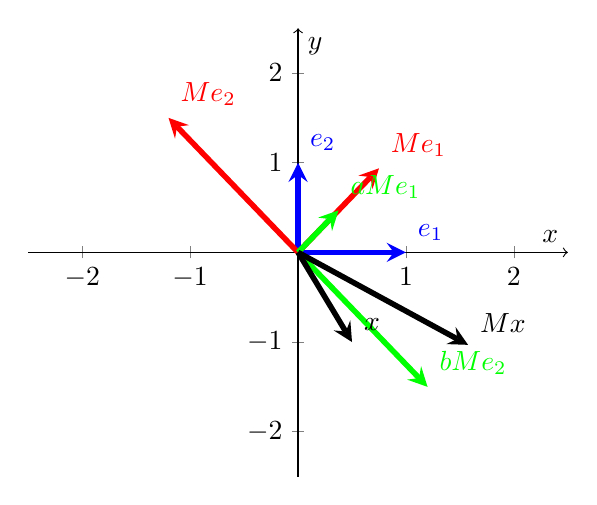
\begin{tikzpicture} 
    \begin{axis}[
        xmin=-2.5,xmax=2.5,
        ymin=-2.5,ymax=2.5,
        axis x line=middle,
        axis y line=middle,
        axis line style=->,
        xlabel={$x$},
        ylabel={$y$},
        ]
\draw[line width=2pt,blue,-stealth](0,0)--(1,0) node[anchor=south west]{$\boldsymbol{e_1}$};
\draw[line width=2pt,blue,-stealth](0,0)--(0,1) node[anchor=south west]{$\boldsymbol{e_2}$};
\draw[line width=2pt,red,-stealth](0,0)--(0.75,0.9375) node[anchor=south west]{$\boldsymbol{Me_1}$};
\draw[line width=2pt,red,-stealth](0,0)--(-1.2, 1.5) node[anchor=south west]{$\boldsymbol{Me_2}$};
\draw[line width=2pt,green,-stealth](0,0)--(0.375,0.46875) node[anchor=south west]{$\boldsymbol{aMe_1}$};
\draw[line width=2pt,green,-stealth](0,0)--(1.2, -1.5) node[anchor=south west]{$\boldsymbol{bMe_2}$};
\draw[line width=2pt,black,-stealth](0,0)--(0.5, -1) node[anchor=south west]{$\boldsymbol{x}$};
\draw[line width=2pt,black,-stealth](0,0)--(1.575, -1.03125) node[anchor=south west]{$\boldsymbol{Mx}$};
    \end{axis}
\end{tikzpicture}
\end{center}
Étant donnés les vecteurs $Me_1$ et $Me_2$, nous savons déterminer l'image de tout vecteur $\begin{bmatrix}
a \\ b
\end{bmatrix}$ : $aMe_1 + bMe_2$, simplement en multipliant $Me_1$ et $Me_2$ par les composantes du vecteur initial, en considérant donc des vecteurs \textit{colinéaires} à $Me_1$ et $Me_2$, puis en additionnant le tout. En plus : $Me_i$ est simplement la $i$ème colonne de $M$. Voyons ceci très explicitement à travers un exemple.\\
$$M = \begin{bmatrix}
3 & -1 \\ 2 & \frac{1}{2}
\end{bmatrix}\text{ et } x = \begin{bmatrix}
-\frac{3}{2} \\ -1
\end{bmatrix}
$$
Calculons d'abord: $Me_1 = \begin{bmatrix}
3 \\ 2
\end{bmatrix}$ et $Me_2 = \begin{bmatrix}
-1 \\ \frac{1}{2}
\end{bmatrix}$, puis $-\frac{3}{2}Me_1 = \begin{bmatrix}
-\frac{9}{2} \\ -3
\end{bmatrix}$ et $-Me_2 = \begin{bmatrix}
1 \\ -\frac{1}{2}
\end{bmatrix}$. Nous devrions obtenir : $Mx = -\frac{3}{2}Me_1 -Me_2 = \begin{bmatrix}
-\frac{9}{2} \\ -3
\end{bmatrix} + \begin{bmatrix}
1 \\ -\frac{1}{2}
\end{bmatrix} = \begin{bmatrix}
-\frac{7}{2} \\ -\frac{7}{2}
\end{bmatrix}$. Vérifions que la géométrie est d'accord :
\begin{center}
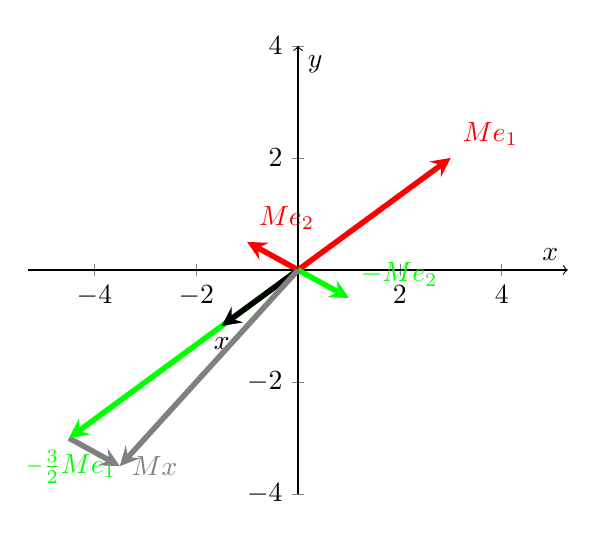
\begin{tikzpicture} 
    \begin{axis}[
        xmin=-5.3,xmax=5.3,
        ymin=-4,ymax=4,
        axis x line=middle,
        axis y line=middle,
        axis line style=->,
        xlabel={$x$},
        ylabel={$y$},
        ]
\draw[line width=2pt,red,-stealth](0,0)--(3,2) node[anchor=south west]{$\boldsymbol{Me_1}$};
\draw[line width=2pt,red,-stealth](0,0)--(-1, 0.5) node[anchor=south west]{$\boldsymbol{Me_2}$};
\draw[line width=2pt,gray,-stealth](-4.5,-3)--(-3.5, -3.5) node[anchor=south west]{};
\draw[line width=2pt,green,-stealth](0,0)--(-4.5,-3) node[anchor=north]{$\boldsymbol{-\frac{3}{2}Me_1}$};
\draw[line width=2pt,green,-stealth](0,0)--(1, -0.5) node[anchor=south west]{$\boldsymbol{-Me_2}$};
\draw[line width=2pt,black,-stealth](0,0)--(-1.5, -1) node[anchor=north]{$\boldsymbol{x}$};
\draw[line width=2pt,gray,-stealth](0,0)--(-3.5, -3.5) node[anchor=west]{$\boldsymbol{Mx}$};
    \end{axis}
\end{tikzpicture}
\end{center}
Nous pouvons alors élargir ce constat aux produits entre matrices, en considérant ici des $2 \times 2$ :
$$AB\begin{bmatrix}
a \\ b
\end{bmatrix} = \begin{bmatrix} Ab_1 & Ab_2 \end{bmatrix}(ae_1+be_2)= a\begin{bmatrix} Ab_1 & Ab_2 \end{bmatrix}e_1 + b\begin{bmatrix} Ab_1 & Ab_2 \end{bmatrix}e_2 = aAb_1 + bAb_2
$$
Notons le rôle similaire joué par $b_1$ et $b_2$ dans la dernière équation. Le produit $AB$ s'assimile alors à une sorte de changement de base, vers celle des colonnes de la matrice $AB$ (attention car ceci n'est pas assimilable à la notion de changement de base que vous verrez en cours).\\
\noindent Si vous désirez des animations ainsi que des explications complémentaires sur l'intuition géométrique en algèbre linéaire, nous vous invitons à regarder \textit{Essence of linear algebra} sur Youtube tout au long du semestre ou avant son début, une playlist réalisée par \textit{3Blue1Brown}, une très belle chaîne de vulgarisation mathématique.


\section{Propriétés des applications matricielles liées aux systèmes linéaires}
%geometric intuition for both surjection and injection: applications that "squish" space (R3->R2, not injective) and applications that "extend" space (R2 -> R3, not surjective)

\subsection{Définition: dépendance et indépendance linéaire}
\begin{boxdef}
Une famille de vecteurs $\{ {v_1},\cdots, {v_n} \}$ de $\R^m$ est dite 
\begin{itemize}
    \item \textit{linéairement indépendante} (ou \textit{libre}) si l'unique combinaison linéaire nulle $ \alpha_1 {v_1} + \cdots + \alpha_n {v_n} = {0}$ est celle pour laquelle $\alpha_1 = \cdots = \alpha_n = 0$
    \item \textit{linéairement dépendante} (ou \textit{liée}) s'il existe des coefficients $\alpha_1,\cdots, \alpha_n $ non tous nuls tels que $ \alpha_1 {v_1} + \cdots + \alpha_n {v_n} = {0}$.
\end{itemize}
\end{boxdef}

\noindent Cela signifie qu'une famille $\{ {v_1},\cdots, {v_n} \}$ est linéairement dépendante si et seulement si un des vecteurs $ {v_1},\cdots, {v_n} $ peut s'écrire comme combinaison linéaire des autres.

\noindent Par exemple, sur $\R^2 $, si une famille contient deux vecteurs colinéaires alors cette famille est linéairement dépendante. À l'inverse, s'ils ne le sont pas alors la famille est linéairement indépendante et génère un plan. De même, sur $\R^3$, si les vecteurs sont coplanaires alors la famille est linéairement dépendante. S'ils ne le sont pas alors la famille est linéairement indépendante et génère un cube.
% \newline On peut donc constater que $n$ vecteurs linéairement indépendants génèrent un espace de dimension $n$.

\noindent Remarquons aussi que la famille $\{ {v_1},\cdots, {v_n} \}$ est linéairement indépendante si et seulement si le système homogène $ A{x} = {0} $, avec $A = \begin{bmatrix} v_1 & v_2 & \cdots & v_n \end{bmatrix}$, ne possède que la solution triviale. En effet, dans $\R^2$ par exemple, si nous avons 2 vecteurs non colinéaires $v_1$ et $v_2$, l'unique façon d'obtenir $\begin{bmatrix} v_1 & v_2\end{bmatrix} x = Ax = 0$ est avec le vecteur nul. Plus généralement, s'il existe des coefficients $\alpha_1, \cdots, \alpha_n$ non tous nuls tels que $\alpha_1 v_1 + \cdots + \alpha_n v_n = 0$, alors $Ax=0$ avec $x = (\alpha_1, \cdots, \alpha_n) \neq 0$.
\newline On peut donc aussi en déduire qu'une famille est linéairement dépendante si et seulement si le système homogène $ A{x} = {0}$ possède des solutions non-triviales (i.e si l'un des vecteurs peut s'écrire comme une combinaison linéaire des autres).

\noindent A noter qu'une famille de vecteurs $\{ {v_1},\cdots, {v_n} \}$ contenant le vecteur nul est toujours linéairement dépendante. En effet, supposons que $ {v_k} = {0} $. On peut écrire
$$ 0\cdot{v_1} + \cdots + 0 \cdot {v_{k-1}} + \alpha \cdot {v_k} + 0 \cdot {v_{k+1}} + \cdots + 0 \cdot {v_n} = {0} $$
avec $ \alpha \in \R$. Les coefficients sont non tous nuls donc une famille contenant le vecteur nul est toujours linéairement dépendante. 

\subsection{Surjectivité d'une application matricielle}
%1 pivot par ligne -> surjective, explain why
\noindent Soit $A \in \R^{p \cross n}$, et soit son application matricielle associée
\begin{align*}
    T: \ &\R^n \to \R^p\\
    &x \mapsto T(x) = Ax
\end{align*}
Rappelons que $T$ est surjective si $\forall b \in \R^p$, $\exists a \in \R^n$ tel que $T(a)=b$. Autrement dit, tout vecteur dans $\R^p$ possède un antécédent dans $\R^n$. Notons que nous n'exigeons aucune condition sur l'unicité de cet antécédent, nous nous intéressons seulement à son existence. \\

\noindent Se poser la question de l'existence d'au moins un $a$ pour tout $b$ dans $\R^p$ tel que $T(a)=b$ revient à étudier le système $Ax=b$, et se demander si pour tout choix de $b \in \R^p$, le système est \textit{compatible}, i.e le système possède toujours une solution. \\

\noindent Avant de répondre à cette question, remarquons que, par la section précédente, la multiplication $Ax$ nous donne un vecteur qui n'est en fait qu'une \textit{combinaison linéaire} des colonnes de $A$. Autrement dit, si $A = \begin{bmatrix} a_1 & \cdots & a_n\end{bmatrix}$ et $x = (x_1, ..., x_n)$, alors:
$$Ax = x_1 a_1 + x_2 a_2 + \cdots + x_n a_n = \sum_{i=1}^{n}x_i a_i$$
Se demander si pour tout choix de $b$, $Ax=b$ possède une solution est donc équivalent à se demander si pour tout choix de $b$, il est possible d'écrire $b$ comme une combinaison linéaire des colonnes de $A$. En effet, les colonnes de $A$ vont \textit{engendrer} un certain espace, que nous appellerons \textit{l'espace colonne} de $A$ et que nous noterons $\Col(A)$ ou encore  défini comme suit :
\begin{boxdef} \label{def:vecteng}
Soient $a_1, \cdots, a_n \in \R^p$. \textit{L'espace engendré} par $a_1, \cdots, a_n$ est noté:
$$\Vect(a_1, ..., a_n) =\left\{b \in \R^p \ | \ \exists (x_1, ..., x_n) \in \R^n \ \sum_{i=1}^n \underbrace{x_i}_{\in \R}\underbrace{a_i}_{\in \R^n} = b\right\} $$
Si $A = \begin{bmatrix} a_1 & a_2 & \cdots & a_n \end{bmatrix} \in \R^{p \times n}$, alors \textit{l'espace colonne} de $A$ est défini comme:
$$\Col(A) = \Vect(a_1, ..., a_n)$$
\end{boxdef}
Remarquons encore que $\Col(A) = \Ima(T)$ où $T$ est l'application matricielle associée à $A$. Ainsi $T$ est surjective, si et seulement si $\Col(A) = \R^p$. \\
Ceci donne une première caractérisation de la surjectivité de $A$. Si $A$ possède plus de lignes que de colonnes (i.e si $A$ est "longue et mince"), $A$ ne pourra jamais être surjective : considérons par exemple la matrice $A = \begin{bmatrix}
a_{1,1} \\
a_{2,1} \end{bmatrix} = \begin{bmatrix}
a
\end{bmatrix}$, qui est composée d'un seul vecteur $a = (a_{1,1}, a_{2,1})$ de $\R^2$, supposons $a_{1,1} \neq 0$ ou $a_{2,1} \neq 0$. Il est impossible que seulement un vecteur de $\R^2$ engendre $\R^2$, i.e il est impossible d'obtenir n'importe quel vecteur de $\R^2$ comme étant une combinaison de ce seul vecteur, il en faut au moins deux. Intuitivement, c'est car $\R^2$ comporte 2 directions, autrement dit que $\R^2$ est \textit{bidimensionnel} et $a$ n'engendre que tout vecteur colinéaire à $a$. \\
Plus précisément : posons $a' = \begin{bmatrix}
-a_{2,1} \\
a_{1,1}
\end{bmatrix}$. Remarquons que le \textit{produit scalaire} de $a$ et $a'$ est nul, autrement dit que les vecteurs $a$ et $a'$ sont \textit{orthogonaux} : $$a \cdot a' = a_1 \times a_1' + a_2 \times a_2' = a_{1,1}\times (-a_{2,1}) + a_{2,1} = 0$$
Géométriquement, $a'$ dirige la droite perpendiculaire à celle dirigée par $a$, ainsi notre intuition devrait nous dire que $a'$ ne peut pas être colinéaire à $a$, et c'est justement cette intuition qui nous pousse ici à poser un tel vecteur $a'$. Vérifions cette intuition \textit{par l'absurde}. Supposons que $a' \in \Vect(a)$, i.e qu'il existe $k \in \R$ tel que $a' = ka$. Puisque $a \neq 0$ (le vecteur nul, $0 = (0,0)$) par hypothèse, alors $a' \neq 0$ alors $k \neq 0$. Ainsi : $$a \cdot a = a \cdot \left(\frac{1}{k}a'\right) = \frac{1}{k}(a \cdot a') = \frac{1}{k} \times 0 \implies a_{1,1}^2 + a_{2,1}^2 = 0 \implies a_{1,1} = a_{2,1} = 0$$
\noindent Nous arrivons à une contradiction puisque nous avons justement supposé que $a_{1,1} \neq 0$ ou $a_{2,1} \neq 0$, ainsi l'hypothèse $a' \in \Vect(a)$ est fausse. Puisqu'il existe un vecteur de $\R^2$ qui n'appartient pas à $\Vect(a)$, $\R^2 \not \subseteq \Vect(a)$, autrement dit $a$ n'engendre pas $\R^2$. \\

\noindent Pour couvrir tous les cas, nous devons encore considérer celui de $a = 0$. Ce cas est dit \textit{trivial}, nous nous rendons facilement compte que : $\Vect(0) = \{b \in \R^2 \ | \ \exists k \in \R\ k0 = b\} = \{0\} \neq  \R^2$.\\ 

\noindent Cette preuve exploitant l'orthogonalité se généralise assez simplement quoiqu'avec des calculs pédagogiquement inutiles donc omis ici, et nous obtenons que :
\begin{boxprop}
Si $A \in \R^{p \cross n}$ avec $p > n$, alors l'application $T(x)=Ax$ ne sera jamais surjective, et $\Col(A) \neq \R^p$.
\end{boxprop}

\noindent Revenons maintenant au système $Ax=b$, et essayons de trouver un critère sur $A$ qui garantisse l'existence d'une solution pour tout choix de $b$. Pour cela, essayons de voir ce qui se passe lorsqu'un système linéaire n'admet pas de solutions. \\
Géométriquement, un système linéaire qui n'admet pas de solutions est un système sur-contraint. C'est un système qui cherche l'intersection de plusieurs droites/plans, alors que cette intersection n'existe pas. Considérons par exemple, dans $\R^2$, le système 
$$\begin{cases} 
x+y=2 & (1)\\
-x+y=1 & (2)\\
x=2 & (3)
\end{cases}$$
qui géométriquement admet comme solution l'intersection des 3 droites, si elle existe. Nous pouvons résoudre ce système avec l'algorithme de Gauss:
$$\begin{bmatrix}
1 & 1 & \bigm| & 2 \\
-1 & 1 & \bigm| & 1 \\
1 & 0 & \bigm| & 3 \\
\end{bmatrix} \sim 
\begin{bmatrix}
1 & 1 & \bigm| & 2 \\
0 & 2 & \bigm| & 3 \\
0 & -1 & \bigm| & 1 \\
\end{bmatrix} \sim 
\begin{bmatrix}
1 & 1 & \bigm| & 2 \\
0 & 2 & \bigm| & 3 \\
0 & -2 & \bigm| & 2 \\
\end{bmatrix} \sim 
\begin{bmatrix}
1 & 1 & \bigm| & 2 \\
0 & 2 & \bigm| & 3 \\
0 & 0 & \bigm| & 5 \\
\end{bmatrix}$$
Regardons la dernière ligne, qui concrètement veut dire que, si $(x,y) \in \R^2$ est solution, alors $0\cdot x + 0\cdot y = 5$, autrement dit que $0=5$, ce qui est contradictoire. Le système ne possède donc pas de solutions, et l'intersection de ces 3 droites n'existe pas. \\
Voici à quoi ressemblent ces 3 droites:
\begin{center}
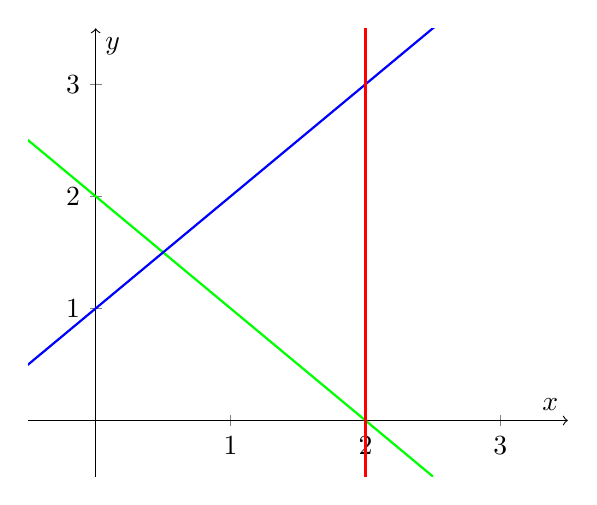
\begin{tikzpicture} 
    \begin{axis}[
        xmin=-0.5,xmax=3.5,
        ymin=-0.5,ymax=3.5,
        axis x line=middle,
        axis y line=middle,
        axis line style=->,
        xlabel={$x$},
        ylabel={$y$},
        ]
    \draw[green, thick] (-1,3) -- (2.5,-0.5);
    \draw[blue, thick] (-2,-1) -- (3,4);
    \draw[red, thick] (2,4) -- (2,-1);
    \end{axis}
\end{tikzpicture}
\end{center}
Il est clair que graphiquement, ce système est incompatible, l'intersection des 3 droites étant non-existante. \\

\noindent Nous avons donc un critère pour assurer l'existence de solutions, notamment l'absence de ligne de $0$ dans la forme échelonnée de la matrice. Comment assurer cela ? En demandant que, dans la forme échelonnée, chaque ligne ait un pivot ! En effet, dans l'absence de ligne de $0$, pour tout choix de $b$ la résolution du système linéaire ne nous donnera aucune contradiction et nous serons capable d'en extraire une solution, ou une famille de solutions. En effet, étant donnée la forme échelonnée réduite suivante :
$$\begin{bmatrix}
1 & 0 & * \bigm| b_1 \\
0 & 1 & * \bigm| b_2
\end{bmatrix}
$$ 
Il sera possible de choisir le vecteur $(x,y,z) = (b_1, b_2, 0)$ comme solution du système linéaire de 2 équations et 3 inconnues associées. Ce raisonnement se généralise aisément à $p$ équations et $n$ inconnues avec une forme échelonnée réduite comptant un pivot sur chaque ligne. Nous aboutissons donc à ce critère :
\begin{boxprop}
$f_A$ est surjective si et seulement si la forme échelonnée de $A$ possède un pivot par ligne.
\end{boxprop}

\subsection{Injectivité d'une application matricielle}
% explain why: chaque colonne comporte 1 pivot <-> injectivité
\noindent Revoyons l'exemple introduit à la toute fin de la section précédente avec la forme échelonnée réduite suivante en spécifiant cette fois-ci quelques valeurs :
$$\underbrace{\begin{bmatrix}
1 & 0 & 5 \\
0 & 1 & 3
\end{bmatrix}}_{A} \begin{bmatrix}
x_1 \\ x_2 \\ x_3
\end{bmatrix} = \underbrace{\begin{bmatrix}
1 \\ 2
\end{bmatrix}}_{b}
$$ 
Nous avons déjà vu comment calculer l'ensemble de solutions de ce système linéaire, nous détaillons néanmoins son calcul :
$$S(A,b) = \left\{\begin{bmatrix}
x_1 \\ x_2 \\ x_3
\end{bmatrix} \ | \ \begin{cases} 
x_1 = -5x_3 + 1 \\
x_2 = -3x_3 + 2
\end{cases} \right\} = \left\{\begin{bmatrix}
-5x_3 + 1 \\ -3x_3 + 2 \\ x_3 + 0
\end{bmatrix} \ | \ x_3 \in \R \right\} = \left\{x_3\begin{bmatrix}
-5 \\ -3 \\ 1
\end{bmatrix} + \begin{bmatrix}
1 \\ 2 \\ 0
\end{bmatrix} \ | \ x_3 \in \R \right\}
$$
Ainsi, pour chaque choix de $x_3$, nous obtenons une nouvelle solution, ainsi $x_3$ est dénommée \textit{variable libre}. Observons que la $3$ème colonne ne comporte pas de pivot.\\

\noindent Nous pouvons remarquer que ceci se généralise et donne une caractérisation des variables libres en termes de pivots : $x_i$ sera une variable libre si et seulement si la $i$ème colonne de la matrice des coefficients ne comporte pas de pivot. S'il existe au moins une variable libre, il y a donc une infinité de solutions au système linéaire $Ax = b$ pour tout $b$, autrement dit la fonction matricielle associée à $A$, $f_A$, est non injective.\\

\noindent Ainsi, $f_A$ injective $\implies$ $A$ admet un pivot sur chaque colonne. \\

\noindent Il est aisé de remarquer que la réciproque est vraie. Si toutes les colonnes de la matrice des coefficients d'un système linéaire admet un pivot, en d'autres termes, que toutes les variables sont \textit{principales} (par opposition à libres), il existe alors au plus un unique choix pour chaque variable afin d'obtenir une solution du système. Exemple :
$$\begin{bmatrix}
1 & 0\\
0 & 1\\
0 & 0\\
\end{bmatrix}\begin{bmatrix}
x_1 \\ x_2
\end{bmatrix} = \begin{bmatrix}
b_1 \\ b_2 \\ b_3
\end{bmatrix} \implies  \text{ La solution existe seulement si }b_3 = 0\text{ et dans ce cas }x_1 = b_1, x_2 = b_2
$$
Ici aussi le constat se généralise simplement. Résumons le critère d'injectivité obtenu :
\begin{boxprop}
$f_A$ est injective si et seulement si sa forme échelonnée compte un pivot par colonne.
\end{boxprop}

Observons de plus le résultat suivant:
\begin{boxthm}
Soit $f$ une application linéaire. Alors
$$\ker(f) = \{0\} \iff f \text{ injective}$$

En particulier, si $A \in \R^{p \cross n}$, alors
$$\ker(A) = \{0\} \iff f_A \text{ injective}$$
\end{boxthm}
\noindent En effet, il semblerait que le vecteur $b = \begin{bmatrix}
1 \\ 2 
\end{bmatrix}$ dans l'exemple introductif de cette section sur l'injectivité n'ait aucune importance, et qu'il aurait pu être remplacé par $(0,0)$. C'est justement le contenu de cette proposition.

\begin{proof}
Exercice 2 de la série 1 !
\end{proof}

% Prouvons cette équivalence en montrant l'implication de chaque côté. \\
% \noindent Pour montrer $\implies$ : Supposons $\ker(A) = \{0\}$, alors $Ax = 0 \implies x = 0$. Ainsi, soient $x_1, x_2 \in \R^n$ tels que $Ax_1 = Ax_2$, alors $A(x_1-x_2) = 0$ et donc $x_1 - x_2 = 0 \implies x_1 = x_2$. Donc $f_A$ est injective.\\
% \noindent Ensuite, pour montrer $\impliedby$ : Supposons que $f_A$ est injective. $A0_{n} = 0_{p}$, avec $0_n \in \R^n$ et $0_p \in \R^p$. Puisque $f_A$ est injective, $\forall x \in \R^n \setminus \{0_n\} \ f_A(x) = Ax \neq A0_n = 0_p$, ainsi $\ker(A)$ ne contient que $0_n$.\\

\noindent Ceci ouvre la discussion de l'intuition géométrique derrière l'injectivité d'applications matricielles. De la même façon qu'une application matricielle $f_M : \R^2 \to \R^3$ ne peut être surjective car $\R^2$ ne pourrait être envoyé qu'au maximum vers un plan de $\R^3$, dirigé par $Me_1$ et $Me_2$ (comme observé à la fin de la section sur le produit matriciel), une application matricielle $f_A: \R^3 \to \R^2$ compresse l'espace tridimensionnel sur (au maximum) un plan bidimensionnel, il ne devrait pas être possible de faire ceci de manière injective avec des applications matricielles.\\

\noindent Nous commençons à comprendre que les fonctions matricielles conservent \textit{certains ensembles} avec des propriétés géométriques intéressantes : si $P$ est un plan de $\R^3$ dirigé par $x$ et $y$ des vecteurs de $\R^3$, $f_A(P)$ pourrait être un plan dirigé par $f_A(x)$ et $f_A(y)$, ou encore une droite si $f_A(y)$ et $f_A(x)$ sont colinéaires, voire même un seul point, l'origine $(0,0)$ si $f_A(v) = (0,0)\ \forall v \in \R^3$.\\

\noindent Dans le cours d'algèbre linéaire, vous définirez précisément ces ensembles - qui sont en fait les \textit{espaces vectoriels}, et qui sont bien plus généraux que des sous-ensembles de $\R^n$.

\subsection{Bijectivité d'une application matricielle}
%the baby of the two above, arrive at the conclusion that the matrix will necessarily be square.
\noindent Pour qu'une application matricielle soit bijective, i.e injective et surjective, il faudra donc, par les deux sections précédentes, qu'elle soit d'abord carrée, puis qu'elle compte un pivot par ligne, ce qui équivalent au fait qu'elle compte un pivot par colonne.\\

\noindent Sa forme échelonnée réduite doit donc être la matrice identité $I_n = \begin{bmatrix}
1 & 0 & \cdots & 0 \\
0 & 1 & \cdots & 0 \\
\vdots & & \ddots& \vdots \\
0 & 0 & \cdots & 1
\end{bmatrix}$.\\
Notons que pour une matrice carrée $A$, il y a 1 pivot par colonne si et seulement s'il y a un pivot par ligne. Ainsi :
\begin{boxthm}
$$A \in \R^{n\times n} \implies \left(f_A \text{ injective } \iff f_A \text{ surjective } \iff f_A \text{ bijective}\right)
$$
\end{boxthm}

\section{Inverse d'une matrice}

\subsection{Motivation, lien avec les applications matricielles}
\noindent Dans les réels, pour les nombres non nuls, nous sommes capables de définir la notion d'inverse. En effet, pour $x \in \R^*$, $\exists y \in \R^*$ tel que $x\cdot y = 1$. Notons $y$ par $x^{-1}$, et appelons-le \textit{l'inverse} de x. Cette notion d'inverse est très commode pour résoudre des équations. Par exemple, pour $x,b \in \R$, $a \in \R^*$, l'équation $ax=b$ peut se résoudre en multipliant par l'inverse de $a$: $x = a^{-1} b$.\\
Nous cherchons à déterminer une notion analogue pour les matrices. Pour $A \in \R^{n \cross p}$, quand est-ce qu'on peut résoudre l'équation $Ax=b$ en écrivant $x = A^{-1}b$ ? Quand est ce que cet inverse existe ? Quelles sont les implications sur la taille de la matrice ? Sur son injectivité, surjectivité ? Comment calculer cet inverse ? \\

\noindent Nous voyons déjà un lien avec l'ensemble des solutions de $Ax=b$. Si cette équation possède une infinité de solutions, il ne sera pas possible d'isoler un seul $x$ comme étant une solution. De plus, si cette équation ne possède aucune solution, il ne sera pas possible non plus d'en extraire un $x$, vu que ce $x$ n'existe pas. Il faut donc que l'équation admette une solution et qu'elle soit unique. Ceci fait le lien avec la bijectivité de l'application matricielle $T(x) = Ax$. Comme vu dans la section précédente, ceci implique que notre matrice est nécessairement carrée, et que l'application est bijective, c'est-à-dire à la fois injective et surjective (et donc que $A$ possède a la fois un pivot par ligne et un pivot par colonne). C'est uniquement dans ce cas que l'inverse d'une matrice peut être défini. Dans ce qui suit dans cette sous-section, $A$ est une matrice carrée de taille $n \cross n$.\\

\noindent Toujours en raisonnant en terme d'applications matricielles, si nous notons $S$ l'application réciproque de $T$ (telle que $S(x) = Bx$, $B \in \R^{n \cross n}$), alors $T\circ S = S \circ T = Id$, c'est-à-dire que la composition de $T$ et de sa réciproque $S$ nous donne l'application identité. Autrement dit, $\forall x \in \R^n$, $(T\circ S)(x) = (S\circ T)(x) = x$, ce qui veut dire que la matrice associée à l'application $T \circ S = S \circ T$ n'est rien d'autre que la matrice identité. \\

\noindent Comme vu précédemment, la composition d'applications matricielles revient à multiplier les matrices associées à ces applications. C'est d'ici que nous obtenons la propriété $AB=BA = I_n$.

\subsection{Définition de l'inverse, quelques propriétés}
\begin{boxdef}
Soit $A \in \R^{n \cross n}$. Si $\exists B \in \R^{n \cross n}$ telle que $AB=BA=I_n$, nous dirons que la matrice $A$ est \textit{inversible} et que la matrice $B$ est son \textit{inverse}, que nous notons $A^{-1}$.
\end{boxdef}

\noindent Cet inverse possède plusieurs propriétés:
\begin{boxprop}
Si $A \in \R^{n \times n}$ est inversible, alors:
\begin{itemize}
    \item L'inverse de $A$ est unique
    \item $(A^{-1})^{-1} = A$
    \item Si $A$ et $B$ sont inversibles, $(AB)^{-1} = B^{-1} A^{-1}$
\end{itemize}
\end{boxprop}

\begin{proof}
Voici une preuve de la première propriété:\\
Supposons qu'il existe deux matrices $B$ et $C$ telles que $AB=BA=AC=CA=I_n$. Alors:
$$B = B\underbrace{I_n}_{=AC} = \underbrace{BA}_{=I_n}C = I_n C = C$$
Les autres propriétés peuvent se prouver en partant de la définition $AB=BA=I_n$, et en identifiant $B$ avec la matrice voulue.

\end{proof}

\noindent Donnons un exemple:
$$\begin{bmatrix} 1 & 2 \\ 0 & 3 \end{bmatrix} \cdot \begin{bmatrix} 1 & -2/3 \\ 0 & 1/3 \end{bmatrix} = \begin{bmatrix} 1\cdot 1 + 2\cdot 0 & 1\cdot -2/3 + 2\cdot 1/3 \\ 0\cdot 1 + 3\cdot 0 & 0\cdot -2/3 + 3\cdot 1/3 \end{bmatrix} = \begin{bmatrix} 1 & 0 \\ 0 & 1 \end{bmatrix} = I_2$$
On notera donc $\begin{bmatrix} 1 & 2 \\ 0 & 3 \end{bmatrix}^{-1} = \begin{bmatrix} 1 & -2/3 \\ 0 & 1/3 \end{bmatrix}$. \\

\noindent Dans ce cours, nous n'avons énoncé qu'une seule manière de déterminer l'existence de l'inverse d'une matrice: le fait que l'application matricielle associée soit bijective, et donc que la matrice de taille $n \cross n$ possède $n$ pivots. Nous avons donc pour le moment cette liste de propositions équivalentes:
\begin{boxthm}
Les propositions suivantes sont équivalentes:
\begin{itemize}
    \item $A \in \R^{n \cross n}$ est inversible
    \item L'application $T: \R^n \to \R^n$, $x \mapsto T(x)=Ax$ est bijective
    \item La forme échelonnée de $A \in \R^{n \cross n}$ possède $n$ pivots
    \item $\ker (A) = \{0\}$
    \item $\Col (A) = \R^n$
\end{itemize}
\end{boxthm}
La taille de cette liste augmentera au fur et à mesure de votre avancement dans le cours d'algèbre linéaire à l'EPFL, lorsque vous étudierez différentes notions qui donnerons différentes caractérisations équivalentes de matrices inversibles. 

\subsection{L'algorithme de Gauss pour trouver l'inverse}
%if u thought u were gonna escape from echelonner then boy you are going to be disappointed with this course
\noindent Soit $A \in \R^{n\cross n}$. Nous avons défini l'inverse de $A$, $A^{-1}$, et nous avons donné quelques propriétés et quelques critères sur son existence. Qu'en est-il de le trouver ? \\

\noindent Rappelons une propriété du produit matriciel, démontrée dans le paragraphe 4.3: \\
En notant $B = \begin{bmatrix} b_1 & \cdots & b_n \end{bmatrix} \in \R^{n \cross n}$, nous avons:
$$AB = \begin{bmatrix} Ab_1 & \cdots & Ab_n \end{bmatrix}$$
De plus, nous avons la propriété $AA^{-1} = I_n$. Pour le moment, notons $A^{-1} = B = \begin{bmatrix} b_1 & \cdots & b_n \end{bmatrix} \in \R^{n \cross n}$, et notons aussi $e_i = (0, ..., 0, \underbrace{1}_{\text{position i}}, 0, ..., 0) \in \R^n$. Notre but est de déterminer $B = A^{-1}$. \\
De cette notation nous obtenons
$$I_n = \begin{bmatrix} e_1 & e_2 & \cdots & e_n \end{bmatrix}$$ 
et par exemple dans $\R^3$, $\{ e_1, e_2, e_3 \} = \left\{ \begin{bmatrix} 1 \\ 0 \\ 0 \end{bmatrix}, \begin{bmatrix} 0 \\ 1 \\ 0 \end{bmatrix}, \begin{bmatrix} 0 \\ 0 \\ 1 \end{bmatrix} \right\}$. \\

\noindent Nous avons donc:
$$AB = I_n \implies \begin{bmatrix} Ab_1 & Ab_2 & \cdots & Ab_n \end{bmatrix} = \begin{bmatrix} e_1 & e_2 & \cdots & e_n \end{bmatrix}$$
Ceci est magnifique. En effet, de cette égalité, nous déduisons que $Ab_1 = e_1$, $Ab_2 = e_2$, et en général, pour $1 \leq i \leq n$, $Ab_i = e_i$. Comme notre matrice $B$ est inconnue, cet ensemble de $n$ systèmes linéaires nous permettent d'expliciter les colonnes de $B$, et donc de la déterminer. Qui dit résoudre une équation matricielle dit algorithme de Gauss et échelonnage. Il faut donc résoudre $n$ systèmes d'équations linéaires de la forme $Ab_i = e_i$, d'inconnue $b_i$, pour déterminer l'inverse de $A$.\\

\noindent Cependant, échelonner la même matrice $n$ fois peut être un peu long, et en effet il existe un raccourci pour trouver l'inverse en échelonnant $A$ qu'une seule fois. En supposant que $Ab_i = e_i$ avec $A$ inversible (donc $f_A$ bijective), $b_i$ est alors l'unique solution de $Ax = e_i$, ainsi :
$$\begin{bmatrix} A & | & e_i\end{bmatrix} \sim \begin{bmatrix} I_n & | & b_i\end{bmatrix}$$
La résolution de ce système nous donne $b_i$, la $i$ème colonne de $B$. Remarquons que, pour cet ensemble de $n$ systèmes, la matrice reste identique, seul le second membre change. Pour éviter d'échelonner $n$ fois, nous pouvons regrouper tous les seconds membres ensemble, comme ceci:
$$\begin{bmatrix} A & | & e_1 & e_2 & \cdots & e_n\end{bmatrix} = \begin{bmatrix} A & | & I_n\end{bmatrix}$$
Nous pouvons ensuite échelonner-réduire $A$ qu'une seule fois pour aboutir à:
$$\begin{bmatrix} I_n & | & b_1 & b_2 & \cdots & b_n\end{bmatrix} = \begin{bmatrix} I_n & | & B \end{bmatrix} = \begin{bmatrix} I_n & | & A^{-1} \end{bmatrix}$$ \\

\noindent Voici donc la méthode pour déterminer l'inverse de $A \in \R^{n \cross n}$ :\\
Commencer par écrire la matrice augmentée:
$$\begin{bmatrix} A & | & I_n\end{bmatrix}$$
Ensuite échelonner-réduire $A$ jusqu'à obtenir la matrice identité à gauche. Le membre de droite correspondra alors à $A^{-1}$:
$$\begin{bmatrix} I_n & | & A^{-1}\end{bmatrix}$$
Notons que si, à gauche, nous n'obtenons pas la matrice identité, alors $A$ n'est pas inversible puisqu'elle n'aura pas, dans ce cas, 1 pivot par colonne.\\

\noindent Illustrons cela avec un exemple. Nous souhaitons calculer l'inverse de $A = \begin{bmatrix} 2 & 1 \\ 1 & 0\end{bmatrix}$: \\
$$\begin{bmatrix} A & | & I_2 \end{bmatrix} = 
\begin{bmatrix}
2 & 1 & \bigm| & 1 & 0 \\
1 & 0 & \bigm| & 0 & 1
\end{bmatrix} \sim 
\begin{bmatrix}
1 & 1/2 & \bigm| & 1/2 & 0 \\
1 & 0 & \bigm| & 0 & 1
\end{bmatrix} \sim
\begin{bmatrix}
1 & 1/2 & \bigm| & 1/2 & 0 \\
0 & -1/2 & \bigm| & -1/2 & 1
\end{bmatrix}$$ 
$$\sim
\begin{bmatrix}
1 & 0 & \bigm| & 0 & 1 \\
0 & -1/2 & \bigm| & -1/2 & 1
\end{bmatrix} \sim 
\begin{bmatrix}
1 & 0 & \bigm| & 0 & 1 \\
0 & 1 & \bigm| & 1 & -2
\end{bmatrix} = \begin{bmatrix} I_2 & | & A^{-1} \end{bmatrix}$$
Ceci nous permet de conclure que $A^{-1} = \begin{bmatrix} 2 & 1 \\ 1 & 0\end{bmatrix} ^{-1} = \begin{bmatrix} 0 & 1 \\ 1 & -2\end{bmatrix}$. \\